\documentclass[]{article}
\usepackage{lmodern}
\usepackage{amssymb,amsmath}
\usepackage{ifxetex,ifluatex}
\usepackage{fixltx2e} % provides \textsubscript
\ifnum 0\ifxetex 1\fi\ifluatex 1\fi=0 % if pdftex
  \usepackage[T1]{fontenc}
  \usepackage[utf8]{inputenc}
\else % if luatex or xelatex
  \ifxetex
    \usepackage{mathspec}
  \else
    \usepackage{fontspec}
  \fi
  \defaultfontfeatures{Ligatures=TeX,Scale=MatchLowercase}
\fi
% use upquote if available, for straight quotes in verbatim environments
\IfFileExists{upquote.sty}{\usepackage{upquote}}{}
% use microtype if available
\IfFileExists{microtype.sty}{%
\usepackage{microtype}
\UseMicrotypeSet[protrusion]{basicmath} % disable protrusion for tt fonts
}{}
\usepackage[margin=1in]{geometry}
\usepackage{hyperref}
\hypersetup{unicode=true,
            pdftitle={DATA 605 - Assignment 5},
            pdfauthor={Joshua Sturm},
            pdfborder={0 0 0},
            breaklinks=true}
\urlstyle{same}  % don't use monospace font for urls
\usepackage{color}
\usepackage{fancyvrb}
\newcommand{\VerbBar}{|}
\newcommand{\VERB}{\Verb[commandchars=\\\{\}]}
\DefineVerbatimEnvironment{Highlighting}{Verbatim}{commandchars=\\\{\}}
% Add ',fontsize=\small' for more characters per line
\usepackage{framed}
\definecolor{shadecolor}{RGB}{248,248,248}
\newenvironment{Shaded}{\begin{snugshade}}{\end{snugshade}}
\newcommand{\KeywordTok}[1]{\textcolor[rgb]{0.13,0.29,0.53}{\textbf{#1}}}
\newcommand{\DataTypeTok}[1]{\textcolor[rgb]{0.13,0.29,0.53}{#1}}
\newcommand{\DecValTok}[1]{\textcolor[rgb]{0.00,0.00,0.81}{#1}}
\newcommand{\BaseNTok}[1]{\textcolor[rgb]{0.00,0.00,0.81}{#1}}
\newcommand{\FloatTok}[1]{\textcolor[rgb]{0.00,0.00,0.81}{#1}}
\newcommand{\ConstantTok}[1]{\textcolor[rgb]{0.00,0.00,0.00}{#1}}
\newcommand{\CharTok}[1]{\textcolor[rgb]{0.31,0.60,0.02}{#1}}
\newcommand{\SpecialCharTok}[1]{\textcolor[rgb]{0.00,0.00,0.00}{#1}}
\newcommand{\StringTok}[1]{\textcolor[rgb]{0.31,0.60,0.02}{#1}}
\newcommand{\VerbatimStringTok}[1]{\textcolor[rgb]{0.31,0.60,0.02}{#1}}
\newcommand{\SpecialStringTok}[1]{\textcolor[rgb]{0.31,0.60,0.02}{#1}}
\newcommand{\ImportTok}[1]{#1}
\newcommand{\CommentTok}[1]{\textcolor[rgb]{0.56,0.35,0.01}{\textit{#1}}}
\newcommand{\DocumentationTok}[1]{\textcolor[rgb]{0.56,0.35,0.01}{\textbf{\textit{#1}}}}
\newcommand{\AnnotationTok}[1]{\textcolor[rgb]{0.56,0.35,0.01}{\textbf{\textit{#1}}}}
\newcommand{\CommentVarTok}[1]{\textcolor[rgb]{0.56,0.35,0.01}{\textbf{\textit{#1}}}}
\newcommand{\OtherTok}[1]{\textcolor[rgb]{0.56,0.35,0.01}{#1}}
\newcommand{\FunctionTok}[1]{\textcolor[rgb]{0.00,0.00,0.00}{#1}}
\newcommand{\VariableTok}[1]{\textcolor[rgb]{0.00,0.00,0.00}{#1}}
\newcommand{\ControlFlowTok}[1]{\textcolor[rgb]{0.13,0.29,0.53}{\textbf{#1}}}
\newcommand{\OperatorTok}[1]{\textcolor[rgb]{0.81,0.36,0.00}{\textbf{#1}}}
\newcommand{\BuiltInTok}[1]{#1}
\newcommand{\ExtensionTok}[1]{#1}
\newcommand{\PreprocessorTok}[1]{\textcolor[rgb]{0.56,0.35,0.01}{\textit{#1}}}
\newcommand{\AttributeTok}[1]{\textcolor[rgb]{0.77,0.63,0.00}{#1}}
\newcommand{\RegionMarkerTok}[1]{#1}
\newcommand{\InformationTok}[1]{\textcolor[rgb]{0.56,0.35,0.01}{\textbf{\textit{#1}}}}
\newcommand{\WarningTok}[1]{\textcolor[rgb]{0.56,0.35,0.01}{\textbf{\textit{#1}}}}
\newcommand{\AlertTok}[1]{\textcolor[rgb]{0.94,0.16,0.16}{#1}}
\newcommand{\ErrorTok}[1]{\textcolor[rgb]{0.64,0.00,0.00}{\textbf{#1}}}
\newcommand{\NormalTok}[1]{#1}
\usepackage{graphicx,grffile}
\makeatletter
\def\maxwidth{\ifdim\Gin@nat@width>\linewidth\linewidth\else\Gin@nat@width\fi}
\def\maxheight{\ifdim\Gin@nat@height>\textheight\textheight\else\Gin@nat@height\fi}
\makeatother
% Scale images if necessary, so that they will not overflow the page
% margins by default, and it is still possible to overwrite the defaults
% using explicit options in \includegraphics[width, height, ...]{}
\setkeys{Gin}{width=\maxwidth,height=\maxheight,keepaspectratio}
\IfFileExists{parskip.sty}{%
\usepackage{parskip}
}{% else
\setlength{\parindent}{0pt}
\setlength{\parskip}{6pt plus 2pt minus 1pt}
}
\setlength{\emergencystretch}{3em}  % prevent overfull lines
\providecommand{\tightlist}{%
  \setlength{\itemsep}{0pt}\setlength{\parskip}{0pt}}
\setcounter{secnumdepth}{0}
% Redefines (sub)paragraphs to behave more like sections
\ifx\paragraph\undefined\else
\let\oldparagraph\paragraph
\renewcommand{\paragraph}[1]{\oldparagraph{#1}\mbox{}}
\fi
\ifx\subparagraph\undefined\else
\let\oldsubparagraph\subparagraph
\renewcommand{\subparagraph}[1]{\oldsubparagraph{#1}\mbox{}}
\fi

%%% Use protect on footnotes to avoid problems with footnotes in titles
\let\rmarkdownfootnote\footnote%
\def\footnote{\protect\rmarkdownfootnote}

%%% Change title format to be more compact
\usepackage{titling}

% Create subtitle command for use in maketitle
\newcommand{\subtitle}[1]{
  \posttitle{
    \begin{center}\large#1\end{center}
    }
}

\setlength{\droptitle}{-2em}
  \title{DATA 605 - Assignment 5}
  \pretitle{\vspace{\droptitle}\centering\huge}
  \posttitle{\par}
  \author{Joshua Sturm}
  \preauthor{\centering\large\emph}
  \postauthor{\par}
  \predate{\centering\large\emph}
  \postdate{\par}
  \date{03/04/2018}


\begin{document}
\maketitle

\begin{Shaded}
\begin{Highlighting}[]
\KeywordTok{library}\NormalTok{(ggplot2)}
\end{Highlighting}
\end{Shaded}

\section{Problem 1}\label{problem-1}

Choose independently two numbers \(B\) and \(C\) at random from the
interval \([0, 1]\) with uniform density. Prove that \(B\) and \(C\) are
proper probability distributions.

Note that the point \((B,C)\) is then chosen at random in the unit
square. Find the probability that:

\subsection{Part 1}\label{part-1}

\indent (a) \(B + C < \frac{1}{2}\)

\subsection{Part 2}\label{part-2}

\indent (b) \(BC < \frac{1}{2}\)

\subsection{Part 3}\label{part-3}

\indent (c) \(|B - C| < \frac{1}{2}\)

\subsection{Part 4}\label{part-4}

\indent (d) \(max\{B,C\} < \frac{1}{2}\)

\subsection{Part 5}\label{part-5}

\indent (e) \(min\{B,C\} < \frac{1}{2}\)

\section{Solutions}\label{solutions}

There are two conditions for the functions to be proper probability
distributions:

\begin{itemize}
\item $\sum P(X = x) = 1$
\item $P(X = x) \geq 0 \ \ \ \ \forall x$
\end{itemize}

\(B\) and \(C\) each have a 100\% probability of \(0 \leq B/C \leq 1\),
so \(B + C\) has a 100\% probability of \(0 \leq B + C \leq 2\).

\begin{Shaded}
\begin{Highlighting}[]
\NormalTok{B <-}\StringTok{ }\KeywordTok{runif}\NormalTok{(}\DataTypeTok{n =} \DecValTok{5000}\NormalTok{, }\DataTypeTok{min =} \DecValTok{0}\NormalTok{, }\DataTypeTok{max =} \DecValTok{1}\NormalTok{)}
\NormalTok{C <-}\StringTok{ }\KeywordTok{runif}\NormalTok{(}\DataTypeTok{n =} \DecValTok{5000}\NormalTok{, }\DataTypeTok{min =} \DecValTok{0}\NormalTok{, }\DataTypeTok{max =} \DecValTok{1}\NormalTok{)}
\end{Highlighting}
\end{Shaded}

\subsection{Part 1}\label{part-1-1}

\indent 1. This is easier to understand visually, so I'll graph the
equation. If we let \(B = x\) and \(C = y\), we can plot the function
\(f(x) = 0.5 - x\).

\begin{Shaded}
\begin{Highlighting}[]
\NormalTok{funcShaded <-}\StringTok{ }\ControlFlowTok{function}\NormalTok{(x) \{}
\NormalTok{    y <-}\StringTok{ }\KeywordTok{seq}\NormalTok{(}\FloatTok{0.5}\NormalTok{,}\DecValTok{0}\NormalTok{, }\DataTypeTok{length.out =} \DecValTok{100}\NormalTok{)}
\NormalTok{    y[x }\OperatorTok{<}\StringTok{ }\DecValTok{0} \OperatorTok{|}\StringTok{ }\NormalTok{x }\OperatorTok{>}\StringTok{ }\FloatTok{0.5}\NormalTok{] <-}\StringTok{ }\OtherTok{NA}
    \KeywordTok{return}\NormalTok{(y)}
\NormalTok{\}}

\NormalTok{function1 <-}\StringTok{ }\ControlFlowTok{function}\NormalTok{(x) }\FloatTok{0.5} \OperatorTok{-}\StringTok{ }\NormalTok{x}
\KeywordTok{ggplot}\NormalTok{(}\DataTypeTok{data =} \KeywordTok{data.frame}\NormalTok{(}\DataTypeTok{x =} \DecValTok{0}\NormalTok{), }\DataTypeTok{mapping =} \KeywordTok{aes}\NormalTok{(}\DataTypeTok{x =}\NormalTok{ x)) }\OperatorTok{+}
\StringTok{  }\KeywordTok{stat_function}\NormalTok{(}\DataTypeTok{fun =}\NormalTok{ function1) }\OperatorTok{+}
\StringTok{  }\KeywordTok{xlim}\NormalTok{(}\DecValTok{0}\NormalTok{, }\FloatTok{0.5}\NormalTok{) }\OperatorTok{+}\StringTok{ }
\StringTok{  }\KeywordTok{ylim}\NormalTok{(}\DecValTok{0}\NormalTok{, }\FloatTok{0.5}\NormalTok{) }\OperatorTok{+}
\StringTok{  }\KeywordTok{stat_function}\NormalTok{(}\DataTypeTok{fun=}\NormalTok{funcShaded, }\DataTypeTok{geom=}\StringTok{"area"}\NormalTok{, }\DataTypeTok{fill=}\StringTok{"#4d535e"}\NormalTok{, }\DataTypeTok{alpha=}\FloatTok{0.2}\NormalTok{)}
\end{Highlighting}
\end{Shaded}

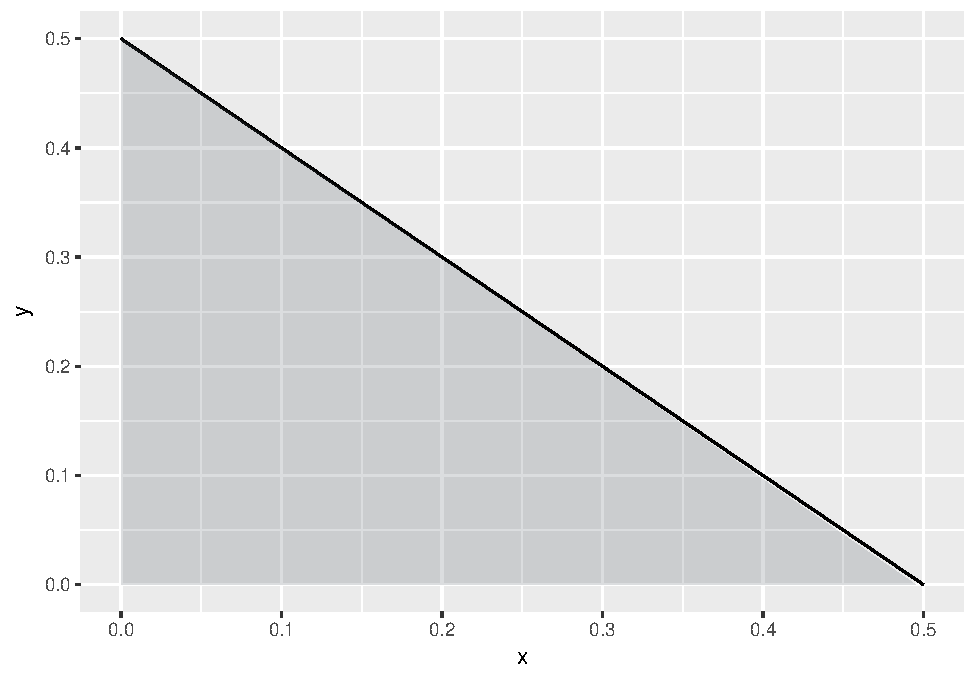
\includegraphics{JSturm_Assignment5_files/figure-latex/unnamed-chunk-1-1.pdf}
The probability that \(x + y < \frac{1}{2}\) is just the area under the
function. In this case, since it's essentially a triangle, we can simply
apply the area formula: \(\frac{1}{2}*\text{base}*\text{height}\).

\begin{Shaded}
\begin{Highlighting}[]
\NormalTok{base <-}\StringTok{ }\FloatTok{0.5}
\NormalTok{height <-}\StringTok{ }\FloatTok{0.5}
\FloatTok{0.5}\OperatorTok{*}\NormalTok{base}\OperatorTok{*}\NormalTok{height}
\NormalTok{## [1] 0.125}
\end{Highlighting}
\end{Shaded}

\subsection{Part 2}\label{part-2-1}

\(xy = \frac{1}{2} \to y = \frac{0.5}{x} \to y = \frac{1}{2x}\).

\begin{Shaded}
\begin{Highlighting}[]
\NormalTok{function2 <-}\StringTok{ }\ControlFlowTok{function}\NormalTok{(x) }\DecValTok{1}\OperatorTok{/}\NormalTok{(}\DecValTok{2}\OperatorTok{*}\NormalTok{x)}
\KeywordTok{ggplot}\NormalTok{(}\DataTypeTok{data =} \KeywordTok{data.frame}\NormalTok{(}\DataTypeTok{x =} \DecValTok{0}\NormalTok{), }\DataTypeTok{mapping =} \KeywordTok{aes}\NormalTok{(}\DataTypeTok{x =}\NormalTok{ x)) }\OperatorTok{+}
\StringTok{  }\KeywordTok{stat_function}\NormalTok{(}\DataTypeTok{fun =}\NormalTok{ function1) }\OperatorTok{+}
\StringTok{  }\KeywordTok{xlim}\NormalTok{(}\DecValTok{0}\NormalTok{, }\DecValTok{1}\NormalTok{) }\OperatorTok{+}\StringTok{ }
\StringTok{  }\KeywordTok{ylim}\NormalTok{(}\DecValTok{0}\NormalTok{, }\DecValTok{1}\NormalTok{) }\OperatorTok{+}
\StringTok{  }\KeywordTok{geom_rect}\NormalTok{(}\KeywordTok{aes}\NormalTok{(}\DataTypeTok{xmin=}\DecValTok{0}\NormalTok{, }\DataTypeTok{xmax=}\FloatTok{0.5}\NormalTok{, }\DataTypeTok{ymin=}\DecValTok{0}\NormalTok{,}\DataTypeTok{ymax=}\DecValTok{1}\NormalTok{), }\DataTypeTok{fill=}\StringTok{"#4d535e"}\NormalTok{, }\DataTypeTok{alpha=}\FloatTok{0.2}\NormalTok{) }\OperatorTok{+}
\StringTok{  }\KeywordTok{stat_function}\NormalTok{(}\DataTypeTok{fun=}\NormalTok{function2, }\DataTypeTok{geom=}\StringTok{"area"}\NormalTok{, }\DataTypeTok{fill=}\StringTok{"#4d535e"}\NormalTok{, }\DataTypeTok{alpha=}\FloatTok{0.2}\NormalTok{)}
\end{Highlighting}
\end{Shaded}

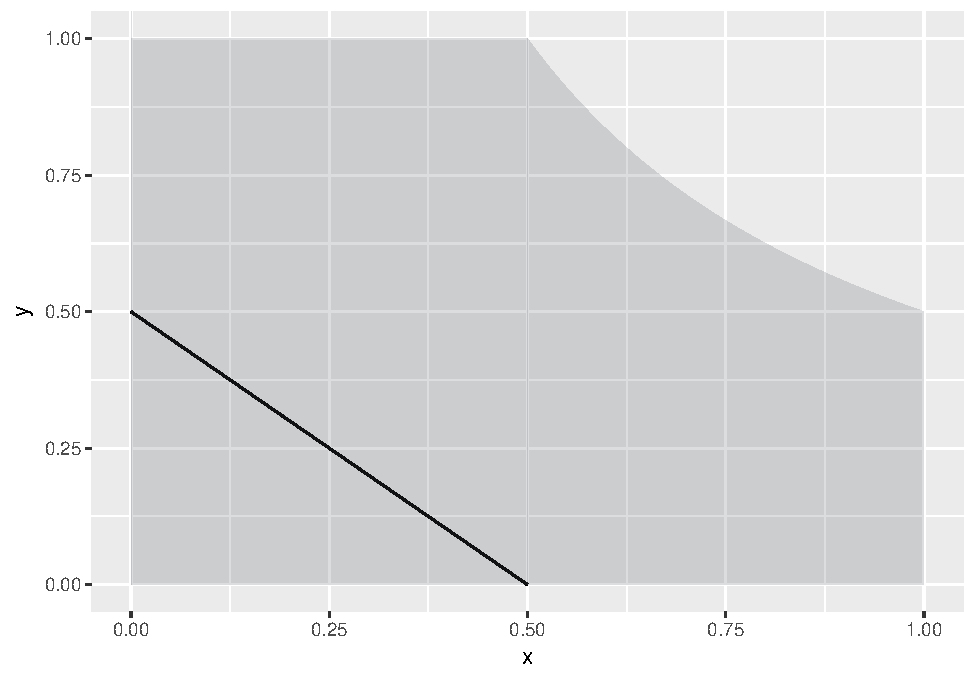
\includegraphics{JSturm_Assignment5_files/figure-latex/unnamed-chunk-3-1.pdf}

Similarly, we need to calculate the area under this curve. We can break
it up into two parts: a rectangle (x=0:0.5, y=0:1) and out function
\(\frac{1}{2x} (x=0.5:1, y=0:\frac{1}{2x}\).\textbackslash{}
\(0.5 * 1 + \int_{0.5}^{1} \frac{1}{2x}dx = 0.846574\).

\begin{Shaded}
\begin{Highlighting}[]
\KeywordTok{integrate}\NormalTok{(function2, }\FloatTok{0.5}\NormalTok{, }\DecValTok{1}\NormalTok{)[[}\DecValTok{1}\NormalTok{]] }\OperatorTok{+}\StringTok{ }\FloatTok{0.5}
\NormalTok{## [1] 0.8465736}
\end{Highlighting}
\end{Shaded}

\subsection{Part 3}\label{part-3-1}

\(|x-y| = \frac{1}{2}\) gives us two lines: \(-x-y = \frac{1}{2}\) and
\(x-y = \frac{1}{2}\).

\begin{Shaded}
\begin{Highlighting}[]
\NormalTok{function3 <-}\StringTok{ }\ControlFlowTok{function}\NormalTok{(x) x }\OperatorTok{+}\StringTok{ }\DecValTok{1}\OperatorTok{/}\DecValTok{2}
\NormalTok{function31 <-}\StringTok{ }\ControlFlowTok{function}\NormalTok{(x) x }\OperatorTok{-}\StringTok{ }\DecValTok{1}\OperatorTok{/}\DecValTok{2}

\NormalTok{shadedx <-}\StringTok{ }\KeywordTok{c}\NormalTok{(}\DecValTok{0}\NormalTok{,}\DecValTok{0}\NormalTok{,}\FloatTok{0.5}\NormalTok{,}\DecValTok{1}\NormalTok{,}\DecValTok{1}\NormalTok{,}\FloatTok{0.5}\NormalTok{)}
\NormalTok{shadedy <-}\StringTok{ }\KeywordTok{c}\NormalTok{(}\DecValTok{0}\NormalTok{,}\FloatTok{0.5}\NormalTok{,}\DecValTok{1}\NormalTok{,}\DecValTok{1}\NormalTok{,}\FloatTok{0.5}\NormalTok{,}\DecValTok{0}\NormalTok{)}
\NormalTok{shadedf <-}\StringTok{ }\KeywordTok{cbind}\NormalTok{(shadedx, shadedy)}

\KeywordTok{ggplot}\NormalTok{() }\OperatorTok{+}
\StringTok{  }\KeywordTok{stat_function}\NormalTok{(}\DataTypeTok{fun =}\NormalTok{ function3) }\OperatorTok{+}
\StringTok{  }\KeywordTok{stat_function}\NormalTok{(}\DataTypeTok{fun =}\NormalTok{ function31) }\OperatorTok{+}
\StringTok{  }\KeywordTok{xlim}\NormalTok{(}\DecValTok{0}\NormalTok{, }\DecValTok{1}\NormalTok{) }\OperatorTok{+}\StringTok{ }
\StringTok{  }\KeywordTok{ylim}\NormalTok{(}\DecValTok{0}\NormalTok{, }\DecValTok{1}\NormalTok{) }\OperatorTok{+}
\StringTok{  }\KeywordTok{geom_polygon}\NormalTok{(}\KeywordTok{aes}\NormalTok{(shadedf[,}\DecValTok{1}\NormalTok{],shadedf[,}\DecValTok{2}\NormalTok{]), }\DataTypeTok{fill=}\StringTok{"#4d535e"}\NormalTok{, }\DataTypeTok{alpha=}\FloatTok{0.2}\NormalTok{) }\OperatorTok{+}
\StringTok{  }\KeywordTok{geom_line}\NormalTok{(}\KeywordTok{aes}\NormalTok{(}\DataTypeTok{x=}\KeywordTok{seq}\NormalTok{(}\DecValTok{0}\NormalTok{,}\FloatTok{0.5}\NormalTok{,}\DataTypeTok{length.out =} \DecValTok{3}\NormalTok{), }\DataTypeTok{y=}\KeywordTok{seq}\NormalTok{(}\FloatTok{0.5}\NormalTok{,}\DecValTok{0}\NormalTok{, }\DataTypeTok{length.out =} \DecValTok{3}\NormalTok{)), }\DataTypeTok{colour =} \StringTok{"#44659b"}\NormalTok{) }\OperatorTok{+}
\StringTok{  }\KeywordTok{geom_line}\NormalTok{(}\KeywordTok{aes}\NormalTok{(}\DataTypeTok{x=}\KeywordTok{seq}\NormalTok{(}\FloatTok{0.5}\NormalTok{,}\DecValTok{1}\NormalTok{,}\DataTypeTok{length.out =} \DecValTok{3}\NormalTok{), }\DataTypeTok{y=}\KeywordTok{seq}\NormalTok{(}\DecValTok{1}\NormalTok{,}\FloatTok{0.5}\NormalTok{,}\DataTypeTok{length.out =} \DecValTok{3}\NormalTok{)), }\DataTypeTok{colour=}\StringTok{"#44659b"}\NormalTok{)}
\end{Highlighting}
\end{Shaded}

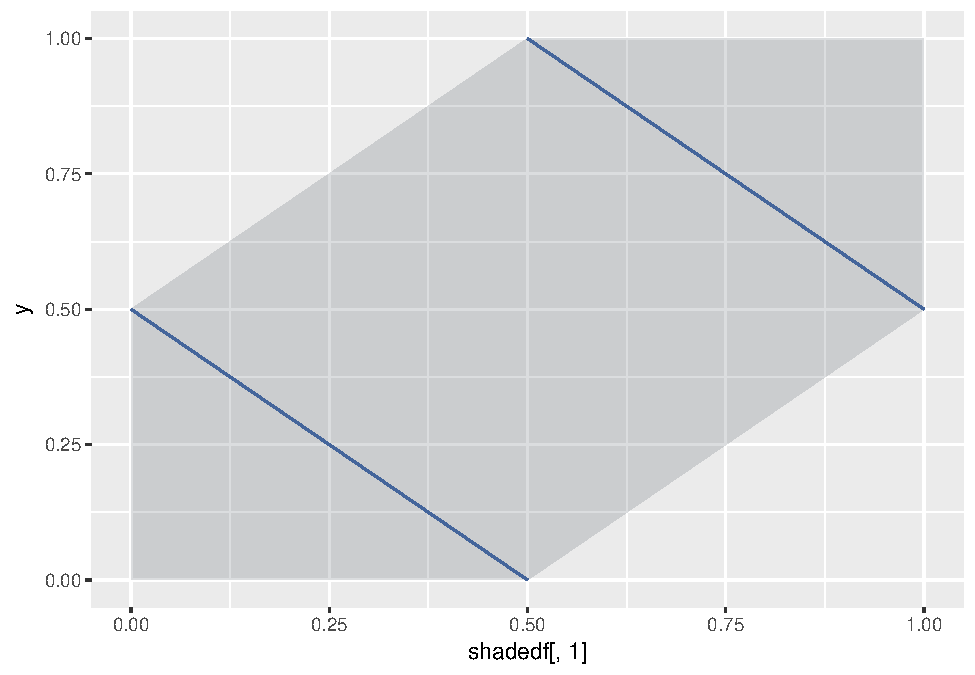
\includegraphics{JSturm_Assignment5_files/figure-latex/unnamed-chunk-5-1.pdf}

The blue lines are not part of the graph, but I included them to better
understand how I approached this problem. Each blue line forms a
triangle, similar to the one we encountered in part a, and also outlines
our unit square. Thus, the area is

\center Area of square - 2 * area of triangle = \(1 - 2*0.25\) = 0.75.

\subsection{Part 4}\label{part-4-1}

\(P(B \leq \frac{1}{2})*P(C \leq \frac{1}{2}) = (\frac{1}{2})^{2} = \frac{1}{4}\).

Alternatively, continuing with the area theme, we could plot the 0.5 by
0.5 square, and its area would be given by \(0.5 * 0.5 = 0.25\).

\begin{Shaded}
\begin{Highlighting}[]
\KeywordTok{ggplot}\NormalTok{() }\OperatorTok{+}
\StringTok{  }\KeywordTok{xlim}\NormalTok{(}\DecValTok{0}\NormalTok{, }\FloatTok{0.6}\NormalTok{) }\OperatorTok{+}\StringTok{ }
\StringTok{  }\KeywordTok{ylim}\NormalTok{(}\DecValTok{0}\NormalTok{, }\FloatTok{0.6}\NormalTok{) }\OperatorTok{+}
\StringTok{  }\KeywordTok{geom_rect}\NormalTok{(}\KeywordTok{aes}\NormalTok{(}\DataTypeTok{xmin=}\DecValTok{0}\NormalTok{, }\DataTypeTok{xmax=}\FloatTok{0.5}\NormalTok{, }\DataTypeTok{ymin=}\DecValTok{0}\NormalTok{,}\DataTypeTok{ymax=}\FloatTok{0.5}\NormalTok{), }\DataTypeTok{fill=}\StringTok{"#4d535e"}\NormalTok{, }\DataTypeTok{alpha=}\FloatTok{0.2}\NormalTok{)}
\end{Highlighting}
\end{Shaded}

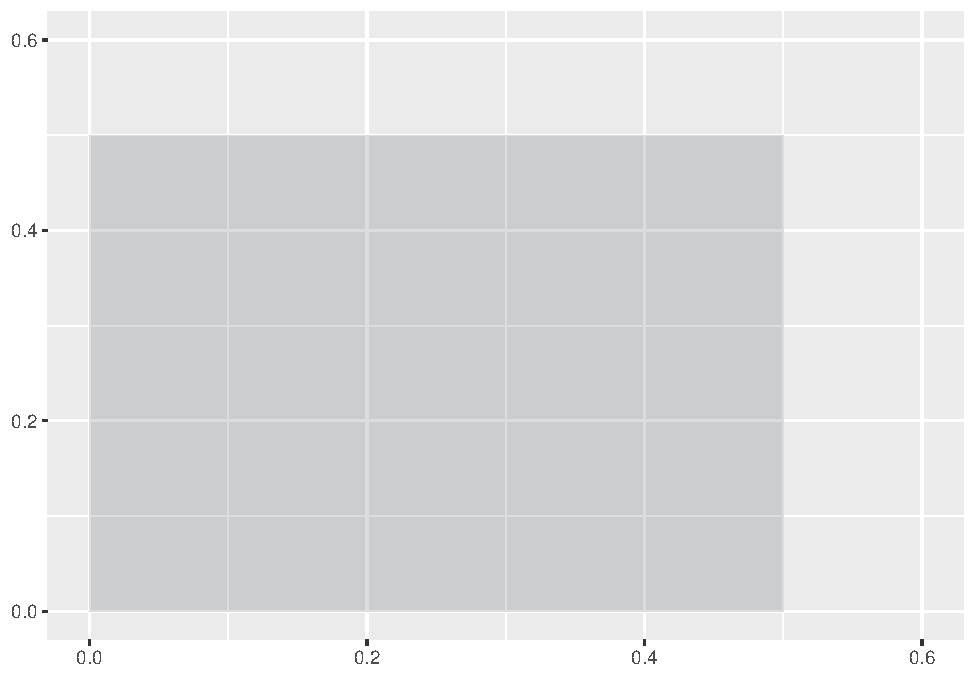
\includegraphics{JSturm_Assignment5_files/figure-latex/unnamed-chunk-6-1.pdf}

\subsection{Part 5}\label{part-5-1}

Either \(B < \frac{1}{2}\) or \(C < \frac{1}{2}\) is needed to satisfy
\(min\{B,C\} < \frac{1}{2}\).

\(P(B < \frac{1}{2} \cup C < \frac{1}{2}) = P(B < \frac{1}{2}) + P(C < \frac{1}{2}) - P(B < \frac{1}{2} \cap C < \frac{1}{2})\).

\(P(B < \frac{1}{2}) = \frac{1}{2}\)

\(P(C < \frac{1}{2}) = \frac{1}{2}\)

\(P(B < \frac{1}{2} \cap C < \frac{1}{2}) = \frac{1}{4}\)

Thus, \(\frac{1}{2} + \frac{1}{2} - \frac{1}{4} = \frac{3}{4} = 0.75\).

\section{References}\label{references}

\begin{itemize}
\tightlist
\item
  \url{https://stackoverflow.com/questions/45301798/ggplot2-how-to-shade-an-area-above-a-function-curve-and-below-a-line}
\end{itemize}


\end{document}
